\documentclass{article}
  \usepackage{amsmath}
  \usepackage{amssymb}
  \usepackage{graphicx}
  \usepackage{float}
  \usepackage{setspace}
\topmargin=-1.2cm \oddsidemargin=0.1cm \evensidemargin=0.1cm
\textwidth=16 true cm \textheight=23 true cm

\font\euler=EUSM10 \font\eulers=EUSM7

\begin{document}
\title{ECON 3160 Game Theory \\Assignment $2^{\text{st}}$, revised}
\author{{\normalsize Leonard Sheng(SHENG, Hao), 1155035947, via \LaTeX}}
\date{\today}

\maketitle

\def \Pr{{\rm Pr}}

\baselineskip 0.6cm
\begin{description}
    \item[3.1:]{\bf Answer:}\\
    {\bf (a):}\\
    The extended belief diagram:\\
    \begin{center}
                    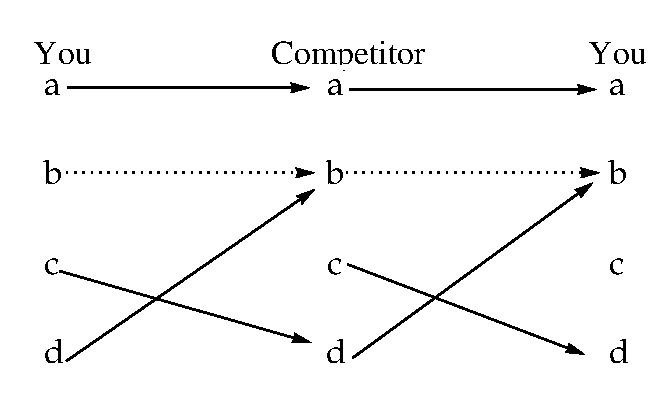
\includegraphics[angle=0, width=0.6\textwidth]{ECON3160A2P1}\\
    \end{center}
    The epistemic model:
    \begin{center}
        \begin{tabular}{cr}
        \hline
        \hline
        \multicolumn{ 1}{c}{{\bf Type}} &          $T_1=\left\{t_1^a,t_1^b,t_1^c,t_1^d\right\}$ \\

        \multicolumn{ 1}{c}{{\bf }} &          $T_2=\left\{t_2^a,t_2^b,t_2^c,t_2^d\right\}$ \\
        \hline
        \multicolumn{ 1}{c}{{\bf Belief of You}} &         $b_1\left(t_1^a\right)=\left(a,t_2^a\right)$ \\

        \multicolumn{ 1}{c}{{\bf }} &         $b_1\left(t_1^b\right)=\left(b,t_2^b\right)$ \\

        \multicolumn{ 1}{c}{{\bf }} &         $b_1\left(t_1^c\right)=\left(d,t_2^d\right)$ \\

        \multicolumn{ 1}{c}{{\bf }} &         $b_1\left(t_1^d\right)=\left(b,t_2^b\right)$ \\\\

        \multicolumn{ 1}{c}{{\bf Belief of Competitor}} &         $b_2\left(t_2^a\right)=\left(a,t_1^a\right)$ \\

        \multicolumn{ 1}{c}{{\bf }} &         $b_2\left(t_2^b\right)=\left(b,t_1^b\right)$ \\

        \multicolumn{ 1}{c}{{\bf }} &         $b_2\left(t_2^c\right)=\left(d,t_1^d\right)$ \\

        \multicolumn{ 1}{c}{{\bf }} &         $b_2\left(t_2^d\right)=\left(b,t_1^b\right)$ \\
        \hline
        \hline
        \end{tabular}
    \end{center}


    {\bf (b):}
    \begin{spacing}{1.0}
    Belief hierarchy of type $t_1^a$:
        \begin{itemize}
          \item you believe your competitor will rationally choose $a$,
          \item you believe your competitor believes that you will rationally choose $a$,
          \item you believe your competitor believes that you believe that he(she) will rationally choose $a$,
        \end{itemize}and so on.\\\\
    Belief hierarchy of type $t_1^b$:
        \begin{itemize}
          \item you believe your competitor will irrationally choose $b$,
          \item you believe your competitor believes that you will irrationally choose $b$,
          \item you believe your competitor believes that you believe that he(she) will irrationally choose $b$,
        \end{itemize}and so on.  \\  \\
    Belief hierarchy of type $t_1^c$:
        \begin{itemize}
          \item you believe your competitor will rationally choose $d$,
          \item you believe your competitor believes that you will irrationally choose $b$,
          \item you believe your competitor believes that you believe that he(she) will irrationally choose $b$,
        \end{itemize}and so on.\\ \\
    Belief hierarchy of type $t_1^d$:
        \begin{itemize}
          \item you believe your competitor will irrationally choose $b$,
          \item you believe your competitor believes that you will irrationally choose $b$,
          \item you believe your competitor believes that you believe that he(she) will irrationally choose $b$,
        \end{itemize}and so on.\\
    \end{spacing}
    {\bf (c):}\\
    Type $t_1^a, t_1^c$ believe in the opponent's rationality.\\
    Among them, only type $t_1^a$ believes that opponent believes in your rationality.\\
    Only type $t_1^a$ expresses common belief in rationality.\\\\
    {\bf (d):}\\
    Only when we start at your choice $a$, we will enter into a cycle of arrows that only reaches rational choices. So, I can only choice $a$ rationally under common belief of rationality. Similarly, for my competitor, he(she) can only choose $a$ rationally under common belief of rationality.\\\\
    {\bf (e):}\\
    The utility form of you and your competitor in the original game:
        \begin{center}
        \begin{tabular}{rcrrrr}

                   &            &             \multicolumn{ 4}{c}{{\bf Competitor}} \\

                   &            &          a &          b &          c &          d \\

        \multicolumn{ 1}{c}{{\bf You}} &          a &  (400,450) &  (500,400) &  (700,200) &  (500,400) \\

        \multicolumn{ 1}{c}{{\bf }} &          b &  (400,500) &  (450,450) &  (400,500) &    (0,900) \\

        \multicolumn{ 1}{c}{{\bf }} &          c &  (200,700) &  (500,400) &  (450,450) &  (500,400) \\

        \multicolumn{ 1}{c}{{\bf }} &          d &  (400,500) &    (900,0) &  (400,500) &  (450,450) \\

        \end{tabular}
        \end{center}
    The reduced game of 1-fold elimination:
        \begin{center}
        \begin{tabular}{rcrrr}

                   &            & \multicolumn{ 3}{c}{{\bf Competitor}} \\

                   &            &          a &          c &          d \\

        \multicolumn{ 1}{c}{{\bf You}} &          a &  (400,450) &  (700,200) &  (500,400) \\

        \multicolumn{ 1}{c}{{\bf }} &          c &  (200,700) &  (450,450) &  (500,400) \\

        \multicolumn{ 1}{c}{{\bf }} &          d &  (400,500) &  (400,500) &  (450,450) \\

        \end{tabular}
        \end{center}
    The reduced game of 2-fold elimination:
        \begin{center}
            \begin{tabular}{rcrr}

                       &            & \multicolumn{ 2}{c}{{\bf Competitor}} \\

                       &            &          a &          c \\

            \multicolumn{ 1}{c}{{\bf You}} &          a &  (400,450) &  (700,200) \\

            \multicolumn{ 1}{c}{{\bf }} &          c &  (200,700) &  (450,450) \\

            \end{tabular}
            \end{center}
        The reduced game of 3-fold elimination:
            \begin{center}
            \begin{tabular}{rcr}

                       &            & {\bf Competitor} \\

                       &            &          a \\

             {\bf You} &          a &  (400,450) \\

            \end{tabular}
            \end{center}
        Thus, after 3 rounds, the algorithm stops. The choices left are exactly same as the answer in Part{\bf (d)}.\\\\
    {\bf (f):}\\Fortunately, the epistemic model given in Part {\bf (a)} is qualified.\\\\
    \item[3.2:]{\bf Answer:}\\
    Let's use some annotation as in Problem 2.2:\\
    In my choices, we denote `C' is choice that I decide to practice Chopin piece for two weeks; `MC' as practice the piece of Mozart for one week and the piece of Chopin for the other, etc.\\
    As for the jury, `MC' means he(she) decides to ask you to play the pieces of Mozart and Chopin in the exam, etc.\\
    {\bf (a):}\\
        The extended belief diagram:
        \begin{center}
                        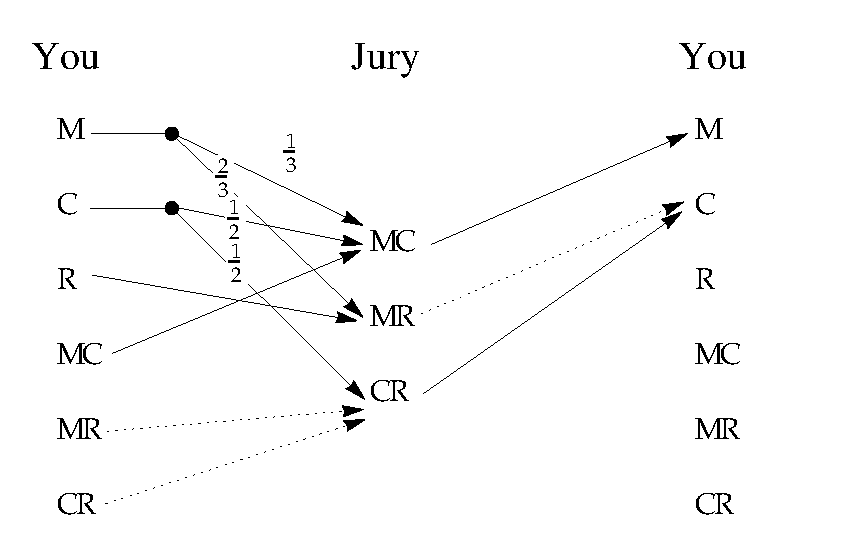
\includegraphics[angle=0, width=0.6\textwidth]{ECON3160A2P2}\\
        \end{center}\newpage
        The epistemic model:
        \begin{center}
                  % Table generated by Excel2LaTeX from sheet 'Sheet1'
            \begin{tabular}{lr}
            \hline
            \hline
            \multicolumn{ 1}{l}{{\bf Type}} &          \multicolumn{1}{l}{$T_1=\left\{t_1^M,t_1^C,t_1^R,t_1^{\text{MC}},t_1^{\text{MR}},t_1^{\text{CR}}\right\}$} \\

            \multicolumn{ 1}{l}{{\bf }} &          \multicolumn{1}{l}{$T_2=\left\{t_2^{\text{MC}},t_2^{\text{MR}},t_2^{\text{CR}}\right\}$} \\
            \hline
            \multicolumn{ 1}{l}{{\bf Belief of You}} &         $b_1\left(t_1^M\right)=\left(\frac{1}{3}\right)\cdot \left(\text{MC},t_2^{\text{MC}}\right)+\left(\frac{2}{3}\right)\cdot \left(\text{MR},t_2^{\text{MR}}\right)$ \\

            \multicolumn{ 1}{l}{{\bf }} &         \multicolumn{ 1}{l}{$b_1\left(t_1^C\right)=\left(\frac{1}{2}\right)\cdot \left(\text{MC},t_2^{\text{MC}}\right)+\left(\frac{1}{2}\right)\cdot \left(\text{CR},t_2^{\text{CR}}\right)$} \\

            \multicolumn{ 1}{l}{{\bf }} &         \multicolumn{ 1}{l}{$b_1\left(t_1^R\right)=\left(\text{CR},t_2^{\text{CR}}\right)$} \\

            \multicolumn{ 1}{l}{{\bf }} &         \multicolumn{ 1}{l}{$b_1\left(t_1^{\text{MC}}\right)=\left(\text{MC},t_2^{\text{MC}}\right)$} \\

            \multicolumn{ 1}{l}{{\bf }} &         \multicolumn{ 1}{l}{$b_1\left(t_1^{\text{MR}}\right)=\left(\text{CR},t_2^{\text{CR}}\right)$} \\

            \multicolumn{ 1}{l}{{\bf }} &         \multicolumn{ 1}{l}{$b_1\left(t_1^{\text{CR}}\right)=\left(\text{CR},t_2^{\text{CR}}\right)$}\\ \\

            \multicolumn{ 1}{l}{{\bf Belief of Jury}} &         \multicolumn{ 1}{l}{$b_2\left(t_2^{\text{MC}}\right)=\left(MC,t_1^{MC}\right)$} \\

            \multicolumn{ 1}{l}{{\bf }} &         \multicolumn{ 1}{l}{$b_2\left(t_2^{\text{MR}}\right)=\left(\text{C},t_1^{\text{C}}\right)$} \\

            \multicolumn{ 1}{l}{{\bf }} &         \multicolumn{ 1}{l}{$b_2\left(t_2^{\text{CR}}\right)=\left(R,t_1^R\right)$} \\
            \hline
            \hline
            \end{tabular}
    \end{center}
    {\bf (b):}\\
     %\begin{spacing}{1.0}
    Belief hierarchy of type $t_1^M$:
            \begin{itemize}
              \item you believe with probability $\frac{1}{3}$, the jury will rationally choose $MC$, that is asking you to play the Mozart and the Chopin;\\
              with probability $\frac{2}{3}$, he(she) will irrationally choose $MR$, that is asking you to play the Mozart and the Rachmaninov;
              \item you believe that the jury believes that, with probability $\frac{1}{3}$, you will rationally choose $MC$, that is to practice the Mozart for one week and the Chopin for the other;\\
              with probability $\frac{2}{3}$, you will rationally choose $C$, that is to practice the Chopin for two weeks,
              \item you believe that the jury believes that you believe that, with probability $\frac{1}{3}$, the jury will rationally choose $CR$;\\
              with probability $\frac{2}{3}$, he(she) will rationally choose $MC$,\\
            and so on.
            \end{itemize}
    Belief hierarchy of type $t_1^C$:
            \begin{itemize}
              \item you believe with probability $\frac{1}{2}$, the jury will rationally choose $MC$, that is asking you to play the Mozart and the Chopin;\\
              with probability $\frac{1}{2}$, he(she) will rationally choose $CR$, that is asking you to play the Chopin and the Rachmaninov;
              \item you believe that the jury believes that, with probability $\frac{1}{2}$, you will rationally choose $R$, that is to practice the Rachmaninov for two weeks;\\
              with probability $\frac{1}{2}$, you will rationally choose $MC$, that is to practice either of the Mozart and the Chopin for one week,
              \item you believe that the jury believes that you believe that, with probability $\frac{1}{2}$, the jury will rationally choose $MC$;\\
              with probability $\frac{1}{2}$, he(she) will rationally choose $CR$,\\
            and so on.
            \end{itemize}
        %\end{spacing}
    {\bf (c):}\\
    Type $t_1^C, t_1^R, t_1^{MC}$ believe in the opponent's rationality.\\
    Among them, all believe that opponent believes in your rationality.\\
    All of type $t_1^C, t_1^R, t_1^{MC}$ express common belief in rationality.\\\\
    {\bf (d):}\\
    When we start at your choices $C, R$ or $MC$, we will enter into a cycle of arrows that only reaches rational choices. So, you can choice $C, R$ or $MC$ rationally under common belief of rationality. Similarly, for the jury, he(she) can chooses both of $MC, CR$ rationally under common belief of rationality.\\\\
    {\bf (e):}\\
    The utility form of you and your competitor in the original game:
        \begin{center}
            \begin{tabular}{rrccc}

                       &            &      \multicolumn{ 3}{c}{{\bf Jury}} \\

                       &            &         MC &         MR &         CR \\

            \multicolumn{ 1}{c}{{\bf You}} &          M & ��6.12,10.12�� & (6.12,9.12) & (4.00,9.00) \\

            \multicolumn{ 1}{c}{{\bf }} &          C & (6.50,10.50) & (4.00,7.00) & (6.50,11.50) \\

            \multicolumn{ 1}{c}{{\bf }} &          R & (4.00,8.00) & (7.00,10.00) & (7.00,12.00) \\

            \multicolumn{ 1}{c}{{\bf }} &         MC & (6.75,10.75) & (5.50,8.50) & (5.25,10.25) \\

            \multicolumn{ 1}{c}{{\bf }} &         MR & (5.50,9.50) & (6.25,9.25) & (4.75,9.75) \\

            \multicolumn{ 1}{c}{{\bf }} &         CR & (5.25,9.25) & (4.75,7.75) & (6.00,11.00) \\

            \end{tabular}
        \end{center}
    The reduced game of 1-fold elimination:
        \begin{center}
            \begin{tabular}{rrcc}

                       &            & \multicolumn{ 2}{c}{{\bf Jury}} \\

                       &            &         MC &         CR \\

            \multicolumn{ 1}{c}{{\bf You}} &          M & ��6.12,10.12�� & (4.00,9.00) \\

            \multicolumn{ 1}{c}{{\bf }} &          C & (6.50,10.50) & (6.50,11.50) \\

            \multicolumn{ 1}{c}{{\bf }} &          R & (4.00,8.00) & (7.00,12.00) \\

            \multicolumn{ 1}{c}{{\bf }} &         MC & (6.75,10.75) & (5.25,10.25) \\

            \end{tabular}
        \end{center}
    The reduced game of 2-fold elimination:
        \begin{center}
            \begin{tabular}{rrcc}

                       &            & \multicolumn{ 2}{c}{{\bf Jury}} \\

                       &            &         MC &         CR \\

            \multicolumn{ 1}{c}{{\bf You}} &          C & (6.50,10.50) & (6.50,11.50) \\

            \multicolumn{ 1}{c}{{\bf }} &          R & (4.00,8.00) & (7.00,12.00) \\

            \multicolumn{ 1}{c}{{\bf }} &         MC & (6.75,10.75) & (5.25,10.25) \\

            \end{tabular}
        \end{center}
    Thus, after 2 rounds, the algorithm stops. The choices left are exactly same as the answer in Part{\bf (d)}.\\\\
    {\bf (f):}\\Fortunately, the epistemic model given in Part {\bf (a)} is qualified.\\\\
    \item[3.4:]{\bf Answer:}\\
    {\bf (a):}\\
    Let $C_B$ denotes the choice of Barbara and $C_C$ denotes the choice of Chris. $C_B, C_C\in$\{0,1,2,3,4,5,6\}, where 1 represents the choice of {\it a}, 2 represents the choice of {\it b}... etc.\\
    The extended belief diagram:
    \begin{center}
                    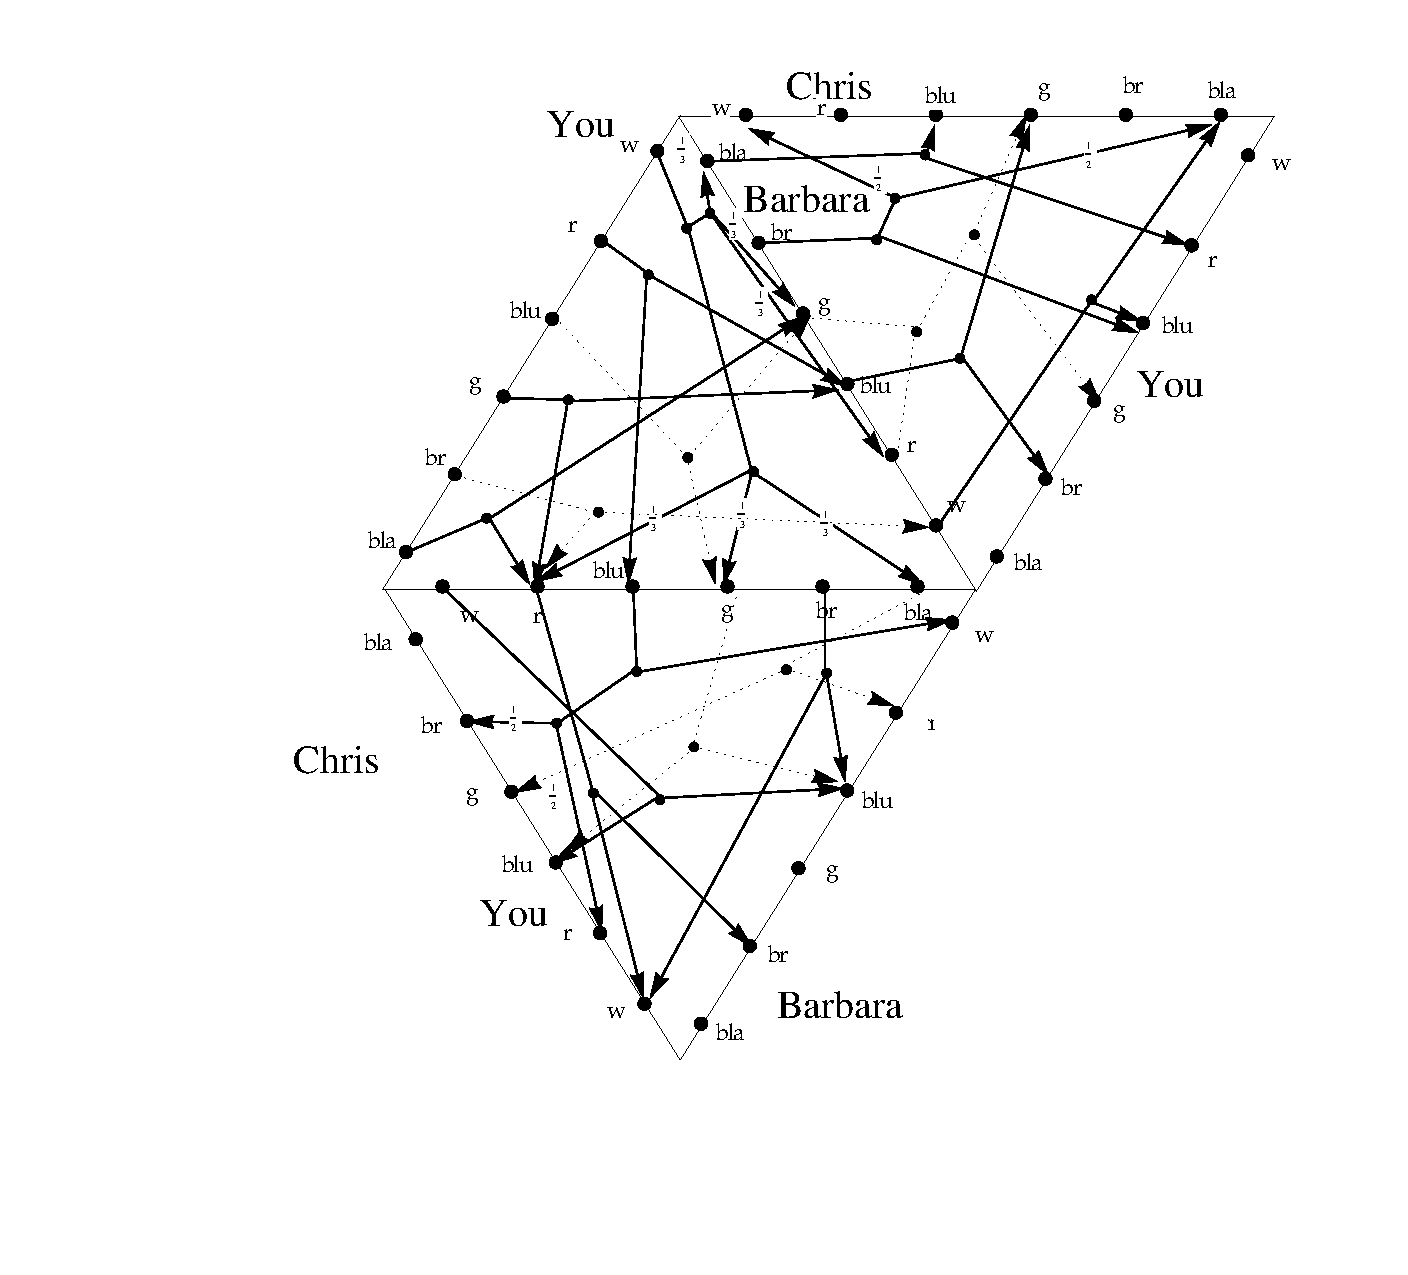
\includegraphics[angle=0, width=0.9\textwidth]{ECON3160A2P3}\\
    \end{center}\newpage
    The epistemic model:
    \begin{center}
        \begin{tabular}{cl}
        \hline
        \hline
        \multicolumn{ 1}{c}{{\bf Type}} &          $T_1=\left\{t_1^{\text{white}},t_1^{\text{red}},t_1^{\text{blue}},t_1^{\text{green}},t_1^{\text{brown}},t_1^{\text{black}}\right\}$ \\

        \multicolumn{ 1}{c}{{\bf }} &          $T_2=\left\{t_2^{\text{white}},t_2^{\text{red}},t_2^{\text{blue}},t_2^{\text{green}},t_2^{\text{brown}},t_2^{\text{black}}\right\}$ \\

        \multicolumn{ 1}{c}{{\bf }} &          $T_3=\left\{t_3^{\text{white}},t_3^{\text{red}},t_3^{\text{blue}},t_3^{\text{green}},t_3^{\text{brown}},t_3^{\text{black}}\right\}$ \\
        \hline
        \multicolumn{ 1}{c}{{\bf Belief of You}} &         $b_1\left(t_1^{\text{white}}\right)=\left(\frac{1}{2}\right)\cdot \left(\left(\text{green},t_2^{\text{green}}\right),\left(\text{black},t_3^{\text{black}}\right)\right)+\left(\frac{1}{2}\right)\cdot \left(\left(\text{red},t_2^{\text{red}}\right),\left(\text{black},t_3^{\text{black}}\right)\right)$\\

        \multicolumn{ 1}{c}{{\bf }} &         $b_1\left(t_1^{\text{red}}\right)=\left(\left(\text{blue},t_2^{\text{blue}}\right),\left(\text{white},t_3^{\text{white}}\right)\right)$ \\

        \multicolumn{ 1}{c}{{\bf }} &         $b_1\left(t_1^{\text{blue}}\right)=\left(\left(\text{green},t_2^{\text{green}}\right),\left(\text{green},t_3^{\text{green}}\right)\right)$ \\

        \multicolumn{ 1}{c}{{\bf }} &         $b_1\left(t_1^{\text{green}}\right)=\left(\left(\text{red},t_2^{\text{red}}\right),\left(\text{red},t_3^{\text{red}}\right)\right)$ \\

        \multicolumn{ 1}{c}{{\bf }} &         $b_1\left(t_1^{\text{brown}}\right)=\left(\left(\text{white},t_2^{\text{white}}\right),\left(\text{red},t_3^{\text{red}}\right)\right)$ \\

        \multicolumn{ 1}{c}{{\bf }} &         $b_1\left(t_1^{\text{black}}\right)=\left(\left(\text{red},t_2^{\text{red}}\right),\left(\text{green},t_3^{\text{green}}\right)\right)$\\ \\

        \multicolumn{ 1}{c}{{\bf Belief of Barbara}} &         $b_2\left(t_2^{\text{white}}\right)=\left(\left(\text{green},t_1^{\text{green}}\right),\left(\text{red},t_3^{\text{red}}\right)\right)$\\

        \multicolumn{ 1}{c}{{\bf }} &         $b_2\left(t_2^{\text{red}}\right)=\left(\left(\text{black},t_1^{\text{black}}\right),\left(\text{green},t_3^{\text{green}}\right)\right)$ \\

        \multicolumn{ 1}{c}{{\bf }} &         $b_2\left(t_2^{\text{blue}}\right)=\left(\left(\text{red},t_1^{\text{red}}\right),\left(\text{white},t_3^{\text{white}}\right)\right)$ \\

        \multicolumn{ 1}{c}{{\bf }} &         $b_2\left(t_2^{\text{green}}\right)=\left(\left(\text{green},t_1^{\text{green}}\right),\left(\text{brown},t_3^{\text{brown}}\right)\right)$ \\

        \multicolumn{ 1}{c}{{\bf }} &         $b_2\left(t_2^{\text{brown}}\right)=\left(\frac{1}{2}\right)\cdot \left(\left(\text{white},t_1^{\text{white}}\right),\left(\text{blue},t_3^{\text{blue}}\right)\right)+\left(\frac{1}{2}\right)\cdot \left(\left(\text{white},t_1^{\text{white}}\right),\left(\text{black},t_3^{\text{black}}\right)\right)$ \\

        \multicolumn{ 1}{c}{{\bf }} &         $b_2\left(t_2^{\text{black}}\right)=\left(\left(\text{blue},t_1^{\text{blue}}\right),\left(\text{blue},t_3^{\text{blue}}\right)\right)$ \\\\

        \multicolumn{ 1}{c}{{\bf Belief of Chris}} &         $b_3\left(t_3^{\text{white}}\right)=\left(\left(\text{red},t_1^{\text{red}}\right),\left(\text{blue},t_2^{\text{blue}}\right)\right)$ \\

        \multicolumn{ 1}{c}{{\bf }} &         $b_3\left(t_3^{\text{red}}\right)=\left(\left(\text{white},t_1^{\text{white}}\right),\left(\text{brown},t_2^{\text{brown}}\right)\right)$ \\

        \multicolumn{ 1}{c}{{\bf }} &         $b_3\left(t_3^{\text{blue}}\right)=\left(\frac{1}{2}\right)\cdot \left(\left(\text{red},t_1^{\text{red}}\right),\left(\text{white},t_2^{\text{white}}\right)\right)+\left(\frac{1}{2}\right)\cdot \left(\left(\text{red},t_1^{\text{red}}\right),\left(\text{brown},t_2^{\text{brown}}\right)\right)$ \\

        \multicolumn{ 1}{c}{{\bf }} &         $b_3\left(t_3^{\text{green}}\right)=\left(\left(\text{blue},t_1^{\text{blue}}\right),\left(\text{blue},t_2^{\text{blue}}\right)\right)$ \\

        \multicolumn{ 1}{c}{{\bf }} &         $b_3\left(t_3^{\text{brown}}\right)=\left(\left(\text{white},t_1^{\text{white}}\right),\left(\text{white},t_2^{\text{white}}\right)\right)$ \\

        \multicolumn{ 1}{c}{{\bf }} &         $b_3\left(t_3^{\text{black}}\right)=\left(\left(\text{red},t_1^{\text{red}}\right),\left(\text{green},t_2^{\text{green}}\right)\right)$ \\
        \hline
        \hline
        \end{tabular}
    \end{center}
    {\bf (b):}\\
    Belief hierarchy of type $t_1^{red}$:
            \begin{itemize}
              \item you believe that Barbara will choose $blue$ and Chris will choose $white$,
              \item you believe that Barbara believes that, you will pick up $red$ and Chris will pick up $white$;
              and you believe that Chris believes that,  you will pick up $red$ and Barbara will pick up $blue$;
              \item you believe that the Barbara believes that you hold the belief that, Barbara will choose $blue$ and Chris will pick up $white$;\\
                  and you believe that the Barbara believes that Chris holds the belief that, Barbara will choose $blue$ and you will pick up $red$;\\
                  and you believe that the Chris believes that you hold the belief that, Barbara will choose $blue$ and Chris will pick up $white$;\\
                  and you believe that the Chris believes that Barbara holds the belief that, Chris will choose $white$ and you will pick up $red$,\\
            and so on.
            \end{itemize}
    Belief hierarchy of type $t_1^{white}$:
        \begin{itemize}
          \item you believe that Chris will choose $black$, and Barbara will choose $red$ or $green$ either with a possibility 50\%,
          \item with possibility 50\%, you believe that Barbara believes that, you will pick up $green$ and Chris will pick up $brown$; with possibility 50\%, you believe that Barbara believes that, you will pick up $blue$ and Chris will pick up $green$;
          and, you believe that Chris believes that, you will pick up $red$ and Barbara will pick up $green$;
          \item with possibility 50\%, you believe that the Barbara believes that you hold the belief that, Barbara will choose $red$ and Chris will pick up $red$; with possibility 50\%, you believe that the Barbara believes that you hold the belief that, Barbara will choose $green$ and Chris will pick up $green$\\
              and with possibility 50\%, you believe that Barbara believes that Chris holds the belief that, Barbara will choose $white$ and you will pick up $white$; with possibility 50\%, you believe that Barbara believes that Chris holds the belief that, Barbara will choose $blue$ and you will pick up $black$\\
              and you believe that the Chris believes that you hold the belief that, Barbara will choose $blue$ and Chris will pick up $white$;\\
              and you believe that the Chris believes that Barbara holds the belief that, Chris will choose $green$ and you will pick up $brown$,\\
        and so on.
        \end{itemize}
    {\bf (c):}\\
    Only the type $t_1^{red}$ expresses common belief in rationality.\\\\
    {\bf (d):}\\
    I will rationally choose $red$ under common belief of rationality. And Barbara will rationally choose $blue$ under common belief of rationality; Chris will rationally choose $white$ under common belief of rationality.\\
    We can reason like this: As is known in the Problem 2.4, I will only rationally choose $red$ and $green$ under belief of opponents' rationality, and Chris will not choose $green$ and $black$ if he is rational, since they only give him utility no more than 2. So, for Barbara, she will get exactly 5 if she chooses $black$, because no one else will choose $black$. Thus, her choice of $white$, $red$, $green$, $brown$ is strictly dominated by the choice of $black$. She will only choose $blue$ or $black$ if she is rational, and holds a belief of her opponents' rationality. Now, for Chris, he will definitely chooses $white$ under common belief of rationality, since in such belief, no one else will pick up $white$. Being aware of this now, I will rationally choose $red$; Barbara will choose $blue$.\\\\
    {\bf (e):}\\
    Well, it's unpractical to list the pay-off pairs of all the $6*6*6$ choices. So we start from the truncated game that all the irrational choice in the original game is eliminated, and my choice of $white$ and $brown$ are also eliminated because of the reason in part {\bf (c)}.\\
    First, we have:
        \begin{center}
            % Table generated by Excel2LaTeX from sheet '3.3'
\begin{tabular}{rrrcccccccc}

           &            & {\bf Barbara:} & \multicolumn{ 2}{c}{white} & \multicolumn{ 2}{c}{blue} & \multicolumn{ 2}{c}{brown} & \multicolumn{ 2}{c}{black} \\

           &            &   {\bf I:} &        red &      green &        red &      green &        red &      green &        red &      green \\

\multicolumn{ 1}{c}{{\bf Chris}} &      white &            &    (6,0,0) &    (5,0,0) &    (6,6,6) &    (5,6,6) &    (6,3,6) &    (5,3,6) &    (6,5,6) &    (5,5,6) \\

\multicolumn{ 1}{c}{{\bf }} &        red &            &    (0,4,0) &    (5,4,4) &    (0,6,0) &    (5,6,4) &    (0,3,0) &    (5,3,4) &    (0,5,0) &    (5,5,4) \\

\multicolumn{ 1}{c}{{\bf }} &       blue &            &    (6,4,3) &    (5,4,3) &    (6,0,0) &    (5,0,0) &    (6,3,3) &    (5,3,3) &    (6,5,3) &    (5,5,3) \\

\multicolumn{ 1}{c}{{\bf }} &      brown &            &    (6,4,5) &    (5,4,5) &    (6,6,5) &    (5,6,5) &    (6,0,0) &    (5,0,0) &    (6,5,5) &    (5,5,5) \\

\end{tabular}
         \end{center}
    Then:
    \begin{center}
      % Table generated by Excel2LaTeX from sheet 'Sheet2'
\begin{tabular}{rrrcccc}

           &            & {\bf Barbara:} & \multicolumn{ 2}{c}{blue} & \multicolumn{ 2}{c}{black} \\

           &            &   {\bf I:} &        red &      green &        red &      green \\

\multicolumn{ 1}{c}{{\bf Chris}} &      white &            &    (6,6,6) &    (5,6,6) &    (6,5,6) &    (5,5,6) \\

\multicolumn{ 1}{c}{{\bf }} &      brown &            &    (6,6,5) &    (5,6,5) &    (6,5,5) &    (5,5,5) \\

\end{tabular}
    \end{center}
    Eventually:
        \begin{center}
          % Table generated by Excel2LaTeX from sheet 'Sheet2'
\begin{tabular}{rrrc}

           &            & {\bf Barbara:} &       blue \\

           &            &   {\bf I:} &        red \\

{\bf Chris} &      white &            &    (6,6,6) \\

\end{tabular}

        \end{center}
    {\bf (f):}\\Fortunately, the epistemic model given in Part {\bf (a)} is qualified.\\\\
    {\bf (g):} {\bf a)}
    The extended belief diagram:
    \begin{center}
                    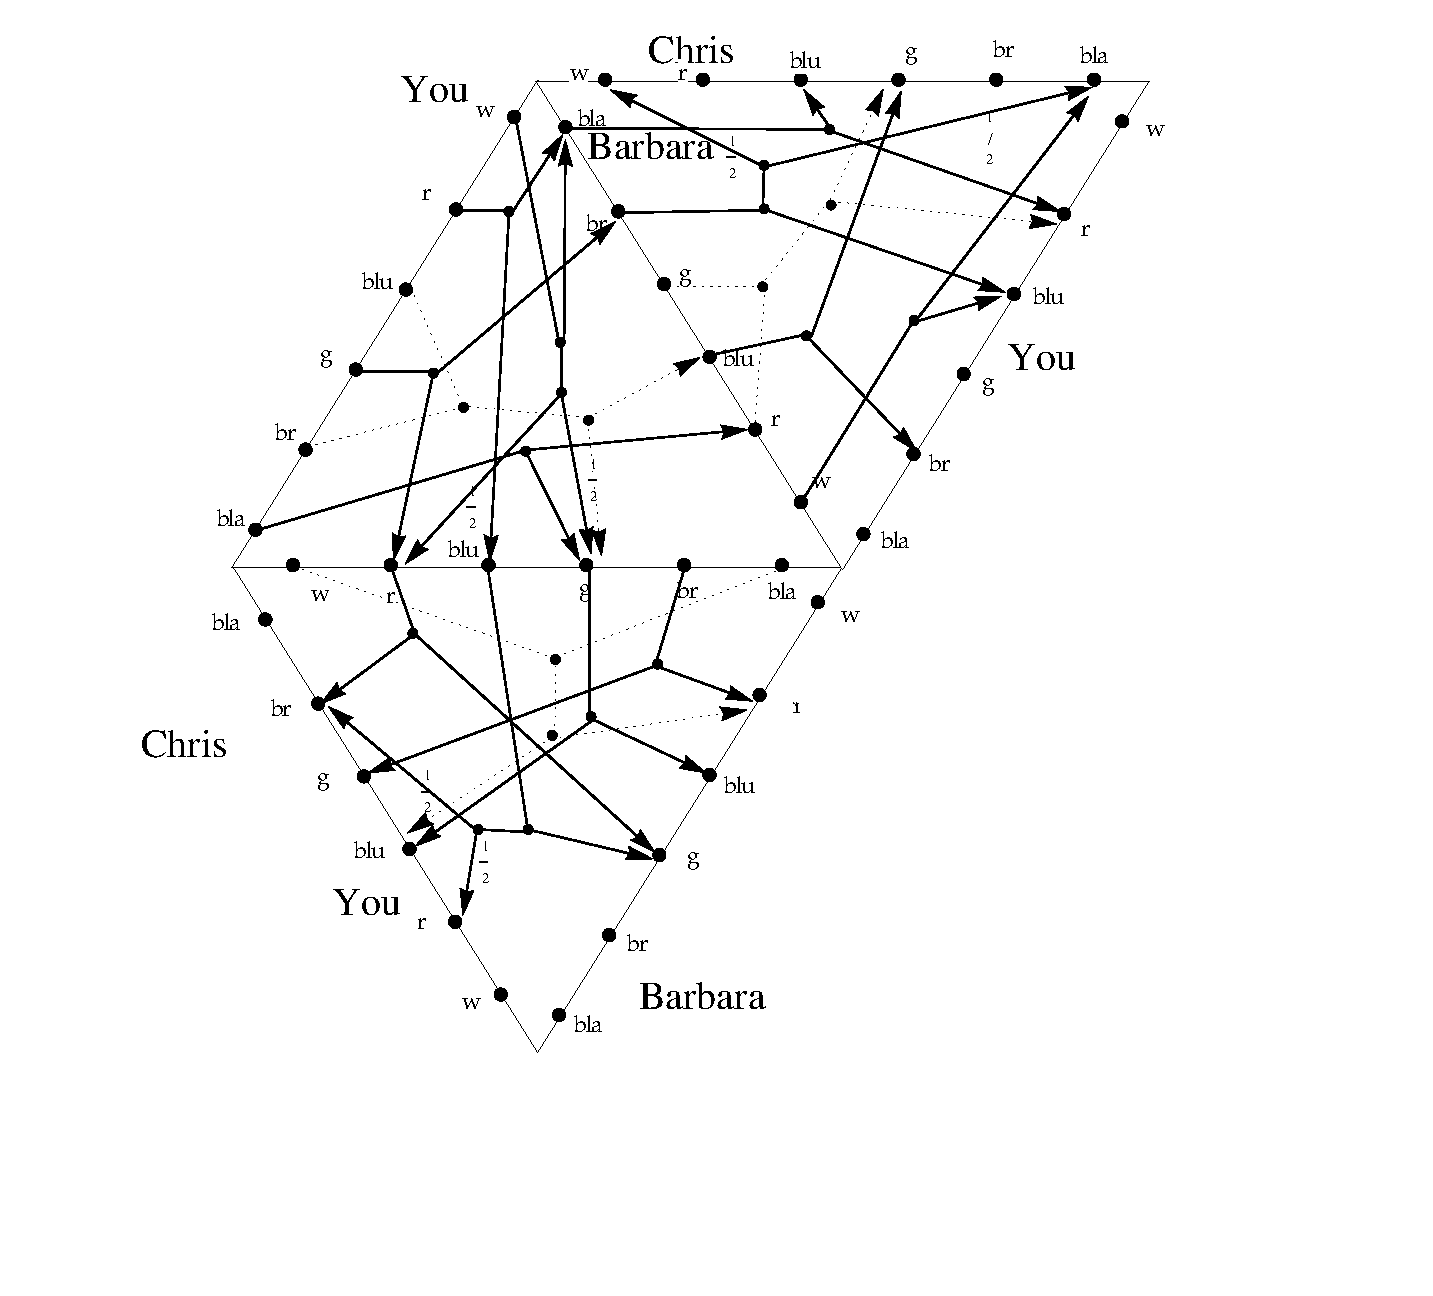
\includegraphics[angle=0, width=0.8\textwidth]{ECON3160A2P4}\\
    \end{center}\newpage
    The epistemic model:
    \begin{center}
        \begin{tabular}{cl}
        \hline
        \hline
        \multicolumn{ 1}{c}{{\bf Type}} &          $T_1=\left\{t_1^{\text{white}},t_1^{\text{red}},t_1^{\text{blue}},t_1^{\text{green}},t_1^{\text{brown}},t_1^{\text{black}}\right\}$ \\

        \multicolumn{ 1}{c}{{\bf }} &          $T_2=\left\{t_2^{\text{white}},t_2^{\text{red}},t_2^{\text{blue}},t_2^{\text{green}},t_2^{\text{brown}},t_2^{\text{black}}\right\}$ \\

        \multicolumn{ 1}{c}{{\bf }} &          $T_3=\left\{t_3^{\text{white}},t_3^{\text{red}},t_3^{\text{blue}},t_3^{\text{green}},t_3^{\text{brown}},t_3^{\text{black}}\right\}$ \\
        \hline
        \multicolumn{ 1}{c}{{\bf Belief of You}} &         $b_1\left(t_1^{\text{white}}\right)=\left(\frac{1}{2}\right)\cdot \left(\left(\text{green},t_2^{\text{green}}\right),\left(\text{black},t_3^{\text{black}}\right)\right)+\left(\frac{1}{2}\right)\cdot \left(\left(\text{red},t_2^{\text{red}}\right),\left(\text{black},t_3^{\text{black}}\right)\right)$\\

        \multicolumn{ 1}{c}{{\bf }} &         $b_1\left(t_1^{\text{red}}\right)=\left(\left(\text{blue},t_2^{\text{blue}}\right),\left(\text{green},t_3^{\text{green}}\right)\right)$ \\

        \multicolumn{ 1}{c}{{\bf }} &         $b_1\left(t_1^{\text{blue}}\right)=\left(\left(\text{blue},t_2^{\text{blue}}\right),\left(\text{green},t_3^{\text{green}}\right)\right)$ \\

        \multicolumn{ 1}{c}{{\bf }} &         $b_1\left(t_1^{\text{green}}\right)=\left(\left(\text{red},t_2^{\text{red}}\right),\left(\text{red},t_3^{\text{red}}\right)\right)$ \\

        \multicolumn{ 1}{c}{{\bf }} &         $b_1\left(t_1^{\text{brown}}\right)=\left(\left(\text{blue},t_2^{\text{blue}}\right),\left(\text{green},t_3^{\text{green}}\right)\right)$ \\

        \multicolumn{ 1}{c}{{\bf }} &         $b_1\left(t_1^{\text{black}}\right)=\left(\left(\text{red},t_2^{\text{red}}\right),\left(\text{green},t_3^{\text{green}}\right)\right)$\\ \\

        \multicolumn{ 1}{c}{{\bf Belief of Barbara}} &         $b_2\left(t_2^{\text{white}}\right)=\left(\left(\text{black},t_1^{\text{black}}\right),\left(\text{blue},t_3^{\text{blue}}\right)\right)$\\

        \multicolumn{ 1}{c}{{\bf }} &         $b_2\left(t_2^{\text{red}}\right)=\left(\left(\text{red},t_1^{\text{red}}\right),\left(\text{green},t_3^{\text{green}}\right)\right)$ \\

        \multicolumn{ 1}{c}{{\bf }} &         $b_2\left(t_2^{\text{blue}}\right)=\left(\left(\text{red},t_1^{\text{red}}\right),\left(\text{green},t_3^{\text{green}}\right)\right)$ \\

        \multicolumn{ 1}{c}{{\bf }} &         $b_2\left(t_2^{\text{green}}\right)=\left(\left(\text{red},t_1^{\text{red}}\right),\left(\text{green},t_3^{\text{green}}\right)\right)$ \\

        \multicolumn{ 1}{c}{{\bf }} &         $b_2\left(t_2^{\text{brown}}\right)=\left(\frac{1}{2}\right)\cdot \left(\left(\text{white},t_1^{\text{white}}\right),\left(\text{blue},t_3^{\text{blue}}\right)\right)+\left(\frac{1}{2}\right)\cdot \left(\left(\text{white},t_1^{\text{white}}\right),\left(\text{black},t_3^{\text{black}}\right)\right)$ \\

        \multicolumn{ 1}{c}{{\bf }} &         $b_2\left(t_2^{\text{black}}\right)=\left(\left(\text{blue},t_1^{\text{blue}}\right),\left(\text{blue},t_3^{\text{blue}}\right)\right)$ \\\\

        \multicolumn{ 1}{c}{{\bf Belief of Chris}} &         $b_3\left(t_3^{\text{white}}\right)=\left(\left(\text{red},t_1^{\text{red}}\right),\left(\text{blue},t_2^{\text{blue}}\right)\right)$ \\

        \multicolumn{ 1}{c}{{\bf }} &         $b_3\left(t_3^{\text{red}}\right)=\left(\left(\text{green},t_1^{\text{green}}\right),\left(\text{brown},t_2^{\text{brown}}\right)\right)$ \\

        \multicolumn{ 1}{c}{{\bf }} &         $b_3\left(t_3^{\text{blue}}\right)=\left(\frac{1}{2}\right)\cdot \left(\left(\text{red},t_1^{\text{red}}\right),\left(\text{green},t_2^{\text{green}}\right)\right)+\left(\frac{1}{2}\right)\cdot \left(\left(\text{red},t_1^{\text{red}}\right),\left(\text{brown},t_2^{\text{brown}}\right)\right)$ \\

        \multicolumn{ 1}{c}{{\bf }} &         $b_3\left(t_3^{\text{green}}\right)=\left(\left(\text{red},t_1^{\text{red}}\right),\left(\text{blue},t_2^{\text{blue}}\right)\right)$ \\

        \multicolumn{ 1}{c}{{\bf }} &         $b_3\left(t_3^{\text{brown}}\right)=\left(\left(\text{green},t_1^{\text{green}}\right),\left(\text{green},t_2^{\text{green}}\right)\right)$ \\

        \multicolumn{ 1}{c}{{\bf }} &         $b_3\left(t_3^{\text{black}}\right)=\left(\left(\text{red},t_1^{\text{red}}\right),\left(\text{blue},t_2^{\text{blue}}\right)\right)$ \\
        \hline
        \hline
        \end{tabular}
    \end{center}
    {\bf b):}\\
    Belief hierarchy of type $t_1^{red}$:
            \begin{itemize}
              \item you believe that Barbara will choose $blue$ and Chris will choose $green$,
              \item you believe that Barbara believes that, you will pick up $red$ and Chris will pick up $green$;
              and you believe that Chris believes that,  you will pick up $red$ and Barbara will pick up $blue$;
              \item you believe that the Barbara believes that you hold the belief that, Barbara will choose $blue$ and Chris will pick up $green$;\\
                  and you believe that the Barbara believes that Chris holds the belief that, Barbara will choose $blue$ and you will pick up $red$;\\
                  and you believe that the Chris believes that you hold the belief that, Barbara will choose $blue$ and Chris will pick up $green$;\\
                  and you believe that the Chris believes that Barbara holds the belief that, Chris will choose $green$ and you will pick up $red$,\\
            and so on.
            \end{itemize}
    Belief hierarchy of type $t_1^{white}$:
        \begin{itemize}
          \item you believe that Chris will choose $black$, and Barbara will choose $red$ or $green$ either with a possibility 50\%,
          \item you believe that Barbara believes that, you will pick up $red$ and Chris will pick up $green$;
           and, you believe that Chris believes that, you will pick up $red$ and Barbara will pick up $black$;
          \item you believe that the Barbara believes that you hold the belief that, Barbara will choose $blue$ and Chris will pick up $green$;\\
              and you believe that Barbara believes that Chris holds the belief that, Barbara will choose $blue$ and you will pick up $red$;\\
              and you believe that the Chris believes that you hold the belief that, Barbara will choose $blue$ and Chris will pick up $white$;\\
              and you believe that the Chris believes that Barbara holds the belief that, Chris will choose $blue$ and you will pick up $blue$,\\
        and so on.
        \end{itemize}
    {\bf c):}\\
    Only the type $t_1^{red}$ expresses common belief in rationality.\\\\
    {\bf d):}\\
    I will rationally choose $red$ under common belief of rationality. And Barbara will rationally choose $blue$ under common belief of rationality; Chris will rationally choose $white$ under common belief of rationality.\\
    After following several arrows, we find that start from that my choices other than $red$ will lead to a dotted arrow finally. My choice $white$ and $brown$ will reach dotted arrows in two rounds. So do my friends.\\\\
    {\bf e):}\\
    We started from the truncated game that all the irrational choice in the original game is eliminated, and my choice of $white$ and $brown$ are also eliminated because of the reason in part {\bf (c)}.\\
    First, we have:
        \begin{center}
         % Table generated by Excel2LaTeX from sheet '3.3.2'
\begin{tabular}{rrrcccccccc}

           &            & {\bf Barbara:} & \multicolumn{ 2}{c}{white} & \multicolumn{ 2}{c}{blue} & \multicolumn{ 2}{c}{brown} & \multicolumn{ 2}{c}{black} \\

           &            &   {\bf I:} &        red &      green &        red &      green &        red &      green &        red &      green \\

\multicolumn{ 1}{c}{{\bf Chris}} &      green &            &     (6,4,6 &    (0,4,0) &    (6,6,6) &    (0,6,0) &    (6,3,6) &    (0,3,0) &    (6,5,6) &    (0,5,0) \\

\multicolumn{ 1}{c}{{\bf }} &        red &            &    (0,4,0) &    (5,4,4) &    (0,6,0) &    (5,6,4) &    (0,3,0) &    (5,3,4) &    (0,5,0) &    (5,5,4) \\

\multicolumn{ 1}{c}{{\bf }} &       blue &            &    (6,4,3) &    (5,4,3) &    (6,0,0) &    (5,0,0) &    (6,3,3) &    (5,3,3) &    (6,5,3) &    (5,5,3) \\

\multicolumn{ 1}{c}{{\bf }} &      brown &            &    (6,4,5) &    (5,4,5) &    (6,6,5) &    (5,6,5) &    (6,0,0) &    (5,0,0) &    (6,5,5) &    (5,5,5) \\

\end{tabular}
         \end{center}
    Then:
    \begin{center}
    % Table generated by Excel2LaTeX from sheet 'Sheet4'
\begin{tabular}{rrrcccc}

           &            & {\bf Barbara:} & \multicolumn{ 2}{c}{blue} & \multicolumn{ 2}{c}{black} \\

           &            &   {\bf I:} &        red &      green &        red &      green \\

\multicolumn{ 1}{c}{{\bf Chris}} &      green &            &    (6,6,6) &    (0,6,0) &    (6,5,6) &    (0,5,0) \\

\multicolumn{ 1}{c}{{\bf }} &      brown &            &    (6,6,5) &    (5,6,5) &    (6,5,5) &    (5,5,5) \\

\end{tabular}
    \end{center}
    Eventually:
        \begin{center}
       % Table generated by Excel2LaTeX from sheet 'Sheet4'
\begin{tabular}{rrrc}

           &            & {\bf Barbara:} &       blue \\

           &            &   {\bf I:} &        red \\

{\bf Chris} &      green &            &    (6,6,6) \\

\end{tabular}

        \end{center}
    {\bf f):}\\Fortunately, the epistemic model given in Part {\bf (a)} is qualified.\\\\
\end{description}
\end{document}
